\documentclass[conference]{IEEEtran}
% The preceding line is only needed to identify funding in the first footnote. If that is unneeded, please comment it out.
\usepackage{url}
\usepackage{amsmath,amssymb,amsfonts}
%\usepackage{algorithmic}
\usepackage{graphicx}
\usepackage{textcomp}
\usepackage{xcolor}
%\usepackage{natbib}
\graphicspath{ {.} }
\def\BibTeX{{\rm B\kern-.05em{\sc i\kern-.025em b}\kern-.08em
T\kern-.1667em\lower.7ex\hbox{E}\kern-.125emX}}

\usepackage{listings}
\usepackage{xcolor}

\usepackage{balance}
 
\definecolor{codegreen}{rgb}{0,0.6,0}
\definecolor{codegray}{rgb}{0.5,0.5,0.5}
\definecolor{codepurple}{rgb}{0.58,0,0.82}
\definecolor{backcolour}{rgb}{0.95,0.95,0.92}

\lstdefinestyle{mystyle}{
    backgroundcolor=\color{backcolour},   
    commentstyle=\color{codegreen},
    keywordstyle=\color{magenta},
    numberstyle=\tiny\color{codegray},
    stringstyle=\color{codepurple},
    basicstyle=\ttfamily\footnotesize,
    breakatwhitespace=false,         
    breaklines=true,                 
    captionpos=b,                    
    keepspaces=true,                 
    numbers=left,                    
    numbersep=5pt,                  
    showspaces=false,                
    showstringspaces=false,
    showtabs=false,                  
    tabsize=2
}
     
\lstset{style=mystyle}

\begin{document}

\title{A Microservices Based Approach for City Traffic Simulation}

\author{\IEEEauthorblockN{1\textsuperscript{st} Toma Becea}
    \IEEEauthorblockA{\textit{Automation and Computer Science Faculty} \\
    \textit{Technical University of Cluj-Napoca}\\
            Cluj-Napoca, Romania \\
            tomabecea@pm.me}
    \and
    \IEEEauthorblockN{2\textsuperscript{nd} Honoriu V{\~a}lean}
    \IEEEauthorblockA{\textit{Automation and Computer Science Faculty} \\
    \textit{Technical University of Cluj-Napoca}\\
            Cluj-Napoca, Romania \\
            Honoriu.Valean@aut.utcluj.ro}
}

\maketitle

\begin{abstract}

The paper proposes a city traffic software simulation based on actors which run independently of one another and have specific characters in their behavior. To run indepentently actors are modeled as microservices and they are running within an orchestration framework. Their behavior is modeled as with specific algorithms for each of their type, embedded in each actor's type code. They may act based on the data about all the other actors, data which is gathered together by a single entity called city simulator. An orchestration model is proposed and all the actors use a communication protocol to offer data to the city simulator and request data from it.

\end{abstract}

\begin{IEEEkeywords}
  traffic simulation; microservices; distributed computing
\end{IEEEkeywords}

\section{Introduction}

A solution which simulates car, pedestrian, etc. traffic in a given city may reap many benefits. It can help understand patterns of traffic and its flow. It can help understand the particularities and pecularities of a city's streets arrangements, together with their junctions. It can help identify bottlenecks. It can help find solutions to rush problems and explore them. But for those areas to be tackled, appropiate methods of simulating traffic must be found and explored. We are proposing a novel way of simulating traffic based on the microservices orchestration concept and using a discrete microscopic logic for the behavior of each actor.

The solution proposed is aiming to design a traffic simulation software which surpasses the computing limits of a single machine and of existing traffic simulation software and runs as a distributed system. In close interplay with the fundamental nature of distributed system (i.e. running a cohesive software on multiple machines) the solution defines entities or actors, modeled as separate microservices, such that the advantage is twofold. First, an entity being a single microservice (and a microservice containing only one entity) they will be easier and natural scheduled and run across more than one machine. Second, the independence of such an entity is also helping in personalize its behavior in randomness and character, offering different ways to model the traffic in a city and allowing more nuanced studies as opposed to macroscopic solutions. This solution can improve a system where only the global state is computed.

We define a \textbf{(city) actor} as being an independent entity which chose to move between two geographical points within a city. As a character, it can be a car, a pedestrian or a bike. We also define the \textbf{city simulator} as being a single entity (subject to distributed and load balacing services) which keeps data about the city (e.g. streets with city actors on them).

\section{Related works}
\label{sec:existingsolutions}

Existing solutions have a general distinction of being scattered across a spectrum: macroscopic, mesoscopic or microscopic being milestones across it. This distinction is caused by how the traffic is modeled: on a macroscopic scale like streets or sections of a highway or on microscopic level, focusing on each car and its relation with neighbours. The relation between a car and its neighbours, can also be modeled as microscopic or nanoscopic.

\cite{abm-for-traffic-routing} describes an Agent Based Model (ABM) for improved traffic routing and achieve a system-optimal traffic flow. The similarity with the current paper is that the data is generating at the agent level and the decision remains at the same level, altough there are two layers in total. First is the microscopic layer which consists of all the intelligent agents. The second layer is the macroscopic layer which facilitates the communications between agents. However, the main difference is that in \cite{abm-for-traffic-routing} an agent is able communicate only with the surrounding ones through the use of cellular automata approach. Agents are communicating a handful of data with their co-participants within a certain range: position, velocity, route and type. Using the data they received they are using a transition decision-making model, based on cellular automata, to compute their next move.

In \cite{8569576} the broad idea is to use a discrete event architecture, in which there are logical processes for executing and simulating a number of agents. For a computation intensive aim those processes can be clustered into agent clusters with dependencies between them, but the paper avoids presenting the necessary details on how the distributed mechanics would work. The particularity of this proposal is that it crosses the boundaries of a single computing machine and pave a way to distribute the load and information across machines, with certain limitations and challenges.

An approach which is focused on junction modeling is \cite{urban-traffic-sim}. As opposed to the generality of various other related works, \cite{urban-traffic-sim} is focused on two specific and real junctions. The simulation stems from SUMO, using real data acquired from cameras placed in junctions (and analyzed with image processing technologies) and is relaying traffic data to a Matlab instance. The simulation is aiming at evaluating metrics of the traffic which flows through junctions: arrival flow and queue length. This idea is closely related to an enhancement proposed in section \ref{sec:enhancements} around junction modeling.

Altough older, \cite{7004985} deserves to be written about because the real data, from the highway portions of interest, is fed back into the simulation. Loop detectors, scattered across the highways are read and their readings are used to generate simulation models. The model is able to predict car densities across multiple road sections, an ability which the current paper is exploring and is basing its car actor's algorithms onto.

\section{Implementation}
\label{sec:implementation}

The entities which are participating into a traffic simulation are called actors. They are two: the city actor and the city simulator. The supporting containers are not themselves part of traffic simulation but they do have an important and supporting role. All of them are modeled as microservices and a short introductory is needed altought section \ref{sec:orchestration} and paragraph \ref{subsec:designchoices} offers a broader perspective around them.

\subsection{Microservices}

Microservices are not a new concept. The idea behind them has existed since Linux kernel has started to be enriched with a concept called namespaces \cite{wiki:linuxns}. This allows one set of processes to see one set of resources while another set of processes see another set of resources, where resources might be, but not limited to, process IDs, file names and network resources. Those linux kernel abilities form the base of containers.

Thus, a container is a small set of processes which run in isolation. They allow packaging a linux distro, a set of libraries and a software development kit and on top of those the custom code of an application. Taken together, those form an image, which is essentially a tar gzipped file. Once the build process of an image is finished, it can be spinned up in one or more running containers. The custom code written and embedded in the image is running in parallel in each container.

To go to solution for building, manipulating and running images is Docker \cite{docker}. It allows easy software installation, it works cross platform and it offers a smooth experience most of the time.

\subsection{City simulator}
\label{subsection:citysimulator}

The most common and easy solution to share data across all the city actors is to have a centralized store to keep it. City simulator acts as a centralized store for all other city actors. In the current implementation the city simulator keeps a set of data which can be described as a list of pairs, each pair having a line and a real number, called density. The line is a series of coordinates and in the proposed implementation their meaning is a street which a city actor is reportedly traveling on it.

The density is defined as the number of actors (cars) which are at a given moment present on a given segment of street. If the city simulator has no entry of a street segment then it will consider the density as being 0, i.e. there is no actor on that street. The density is modeled as an unsigned integer.

Fig. \ref{fig:citysimrelations} depicts the city simulator in relation with the other entities. A notable exception is the web page. Its purpose is not to participate in the same information exchange the other entities have but to offer a visual interpretation about the way the city and the other actors are interacting with one another.

\begin{figure}
    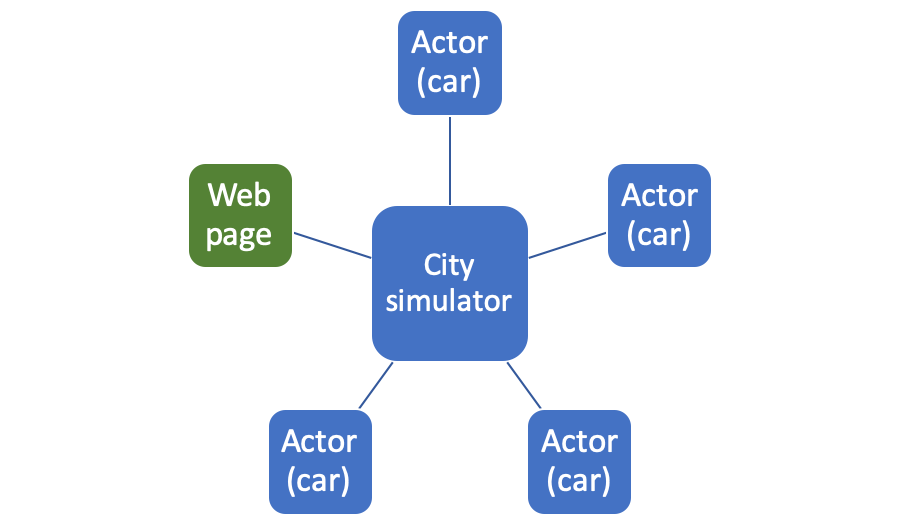
\includegraphics[width=8cm]{CitySimulator.png}
    \centering
    \caption{The relations of city simulator with other entities}
    \label{fig:citysimrelations}
\end{figure}

As various actors send data about their location, the city simulator needs to keep location and density data in its store. It does not know of Open Street Map maps and its corresponding map data sets but instead it requires any actor to send its current set of coordinates which it is crossing or which it left. If any other actor send the same set of coordinates, or a subset of it then the first set of coordinates will have its density incremented. Listing \ref{lst:goactorstruct} shows the Go struct which is used by an actor to send its report to the city simulator and is used by the city simulator to decode a message received from an actor. Apart from this line there are two more details to complete the report picture. Listing \ref{lst:goactorreports} contains the type of communications between actors and the citysimulator.

\begin{lstlisting}[caption=Go struct for actor's report, label=lst:goactorstruct]
// Report is the base type for reporting
// status and vectors to a city entity
type Report struct {
	CurrentLine  [][]float64
	ReportDetail int
}
\end{lstlisting}

As part of this proposal the city simulator is made to be a standalone entity (container) which communicates with actors. This might not be the case for other types of communications, as part of other architectures. One example can be the integration or the unifying of the city simulator with the city actor, both becoming one entity. In this case the communication between entities is subject to an entire panoply of choices.

\subsection{Car actor}

The city actor represents a moving actor within a city. It can be a car which moves across the city, it can be a bike or it can be a pedestrian. Its naming suggests that it can be any entity or living being which moves within a city and interacts with the other entities or affects the other entities in some manner. A pedestrian would directly interact with other pedestrians but not with cars unless it crosses the street on red or on unmarked places. A pedestrian would indirectly affect other cars by willing to walk over a street crossing.

The implementation proposed here is aiming to model a single type of actor: a car which moves between two points across a city. Because the purpose of this paper is not to tackle maps representation and routing through a city (in itself, this area is way bigger than a mere technical paper) the city actor is using two notable services: Open Street Map \cite{openstreetmap} and GraphHopper \cite{graphhopper}. Open Street Map is an open source licensed map of the entire world. Graphhoper is an open source service which offers directions APIs and route planning. It can use Open Street Map as an underlying map provider. They provide free tiers and paid subscription for accessing an API and compute various routes. However, a city actor is not using any public api but a special crafted container which contains GraphHopper and an open street map embedded into it. Thus, this container is running in parallel with the other city actors and provides them with the routing API they need.

A first way to introduce randomness into the entire simulation of a city is to choose a set of two coordinates inside the given city, a set for each city actor. Then the actor proceeds to ask GraphHopper service for a route between those two points. Because each city actor 'lives' only while its moving across its route and 'dies' as soon as it reached the finish point, the entire city simulation which takes place is made of independent, random and always new actors.

\subsection{Interactions}

An actor interacts, for the time being, only with the city simulator by using a Go struct and a Go enum. They can be seen in listings \ref{lst:goactorstruct} and \ref{lst:goactorreports}. The message sent from one side to another has a general structure called \textit{Envelope}. It is meant to offer a top level message which can be serialized (or encoded, the way to do this in Golgang, if not gRPC, is the gob pacakge offered out of the box as a base package within the lanugage) and passed around, enabling any party involved to understand what this message is about and how to decode it.

Listing \ref{lst:goenvelope} show the top level message. It contains a message type which instructs the reader what kind of message it has to deal with and the possible types are the second part of listing \ref{lst:goactorstruct}: \textit{SendReport}, \textit{AskForLine}, \textit{RespondWithLine}. Let's take them one by one. \textit{SendReport} represents a message sent from an actor to the city simulator and the \textit{Payload} contains the report seen in listing \ref{lst:goactorreports}. 

\textit{AskForLine} is a message sent from an actor to the city simulator in which the actor asks about the density of any line. This way any actor can take conscious decisions on which route to go on, based on what lies ahead in terms of street densities. When a first route is chosen, between two desired points, the actor can ask about each line which is part of that route. The city simulator will respond with the known density of it. If the actor desires, it can try to find another route by asking GraphHopper service to compute a new route but with an additional rule: avoid a certain point (street, junction, etc.). \textit{RespondWithLine} is the type of message which the city simulator sends back to an actor after it received an \textit{AskForLine} message.

\begin{lstlisting}[caption=Go enumerations for messaging, label=lst:goactorreports]
const (   
    // ReportOnTheLine is the report sent by one agent to
    // notify the city that he is currently advancing
    // through one line.
    ReportOnTheLine = iota
    
    // ReportOffFromLine is the report sent by one agent to
    // notify the city that he has finished advancing through
    // one line and has departed from it.
    ReportOffFromLine = iota
)
    
const (
    // SendReport is a message passed from an actor to the city
    // indicating its status (e.g. location).
    SendReport = iota
    
    // AskForLine is a message passed from an actor to the city.
    // A response is awaited.
    AskForLine = iota
    
    // RespondWithLine is a message passed from the city to
    // an actor and it contains line data.
    RespondWithLine = iota
)
\end{lstlisting}

\begin{lstlisting}[caption=Go top level struct (envelope), label=lst:goenvelope]
// Envelope is the container for different messages sent back
// and forth between an actor and a city
type Envelope struct {
    MessageType int
    Payload     interface{}
}
\end{lstlisting}

\subsection{Design choices}
\label{subsec:designchoices}

As with every software project started from scratch there are a number of choices to make when choosing software stacks, programming languages, networking models, etc. This section is aiming to explore the rationales behind some of those decisions and how they influenced the building of the current prototype.

A first choice is the programming language to write both the city simulator and the city actor. Go programming langauge is born out of Google and it resembles the philosophy they were trying to embedded in it for taming the complexity of their systems \cite{donovan2015go}. Today it has gained a lot of popularity and tools like Kubernetes are wrritten entirely in Go, making it the default language of the cloud technologies. It is a "C-like" language and it has a familiar look but with few traits which makes it different. Out of those, few are notable, not only because they facilitate programming endeavors but also because both city simulator and city actor are modeled around them in their communications. 

\begin{lstlisting}[caption=Go routine from city actor, label=lst:goroutine]
go func() {
	for {
		select {
		case <-ticker.C:
			advance(city, reportChan, lineChan)
		case _ = <-lineChan:
			//fmt.Println("Received answer with line", j)
		}
	}
}()
\end{lstlisting}

Go routines are a lightweight thread of executing. Being lightweight it means they can be easily started, with no overhead and especially without the ceremony of dealing with threads which other popular languages (e.g. Java) have. Listing \ref{lst:goroutine} shows such a routine. It is a part of logic where the city actor responds to either two events: the timer has expired and a decision needs to be made or an information about the line is currently traveling on has been received from the city simulator. Another Go trait is the channels, an indexed communication pipe where there are asynchronous writers and readers, used to decouple two routines. Listing \ref{lst:goroutine} also shows couple of channels. Variables \textit{ticker} and \textit{lineChan} are two channels. They are declared using a type and after that they are used to write and read objects (or structs) of the respective type. The \textit{select} keyword acts like a switch, not on variables and their values but on channels. It will execute the block of code for the channel which has something new to deliver. All those three concepts, \textit{goroutines}, \textit{channels} and \textit{select} switches, combined together makes it easy to write code which takes advantage of multithreading paradigms and which has to run in a heavy networking environment.

\section{Orchestration}
\label{sec:orchestration}

The term orchestration means the handling of containers and microservices in order to bring coherence into their interaction and an unifying experience to the end user of a service or of a product. They migth run on multiple nodes (computers or virtual machines) and at the same time they need to communicate with one another. They need to be updated in place and without service disruption. Whenever one of them crash they have to restart as quickly as possible. The services have to be able to discover themselves without dealing with intricancies of IP addresses, proxies, etc. Those are just few concerns around orchestration and the current paper is not aiming to provide a comprehensive view of what it means and what can be achieved with it but rather to set a basis of understanding enough context for the subject of simulating a city with its traffic.

\cite{7922500} offers a comprehensive view of the current state of orchestration of cloud providers. (to add details)

\subsection{Current state}

As noted above the standard in easiness of developing and working with containers is Docker \cite{docker}. While it has an offering of orchestrating containers, called \textit{docker-compose}, which is simple to start with, its functionality is limited in comparison with other offerings, the most notable one being Kubernetes \cite{Kubernetes}. Those are not the single tools available and many more can be found but they offer a starting point (especially Docker) and Kubernetes, altough it has a steep learning curve, it does offer a comprehensive and complex panoply of details around orchestration.

\subsection{Implementation}

The city simulator is, currently, a single service which means it runs as a single instance as viewed by a city actor. The city actor container runs in multiple instances and it has the need to do so as part of the entire simulation workload. The other two instances which run in the simulation are the routing service, a Graphhopper instance, and the front end web erver which displays a web page for offering visual clues about how the simulation is running. While they run as such there should be an easy way, without friction and additional compute logic to "discover" a certain service. A city actor will need to connect itself to the routing service and to the city simulator. At the same time the front end instance need to connect itself to the city simulator to source its data.

\subsection{Docker compose}

The \textit{docker-compose} tool gives the ability to manipulate more containers and services, with a simple file written in yaml format. Listing \ref{lst:dockercompose} shows the docker-compose file in its brevity and briefness. Let's dissect it. There are four services: \textit{graphhopper}, \textit{citysim}, \textit{cityactor} and \textit{cityfront}. Each of them need an image to run and this image can be specified in two ways: either as an image already compiled and hosted on an container registry or as a local folder which contains a file to build one (usually named \textit{dockerfile}). Because Graphhoper, once compiled with desired maps and settings do not need any more development work, it is uploaded to a personal docker registry and taken from there, whenever needed. The other three services are the places where the most development efforts take place therefore they need to be compiled or recompiled each time the entire traffic simulation application starts.

The containers which are running may need to have different properties. First and most important is the container port which needs to be published. The port from inside the container, where a certain process expect a TCP communication is forwarded to the local host port and thus is accessible from outside the Docker internal network. Another detail of the container is its dependency. For example \textit{cityactor} cannot run without textit{Graphhopper} because it doesn't have any place to obtain a route. Therefore it depends on \textit{Graphhopper}, i.e. it waits for GraphHopper to start first. And on \textit{citysim}, of course. The last bit of detail which can be seen here is the policy of restarting a container. By default the policy is set to "No" which means that the container will not be restarted if there is any failure within it and it stops. However, for simulation purposes, as we need a constant stream of city actors to swarm through the city, the policy is set to "Always" which will restart the container after if closes itself, i.e. it finishes its travel.

\begin{lstlisting}[caption=Docker-compose file, label=lst:dockercompose]
services:
  graphhopper:
    image: tomabecea/graphhopper:latest
    ports:
      - "8989:8989"
  citysim:
    build: ./city/citysim
    ports:
      - "9000:9000"
  cityactor:
    build: ./city/cityactor
    depends_on: 
      - "graphhopper"
    restart: always
  cityfront:
    build: ./cityfront
    ports:
      - "80:80"
    depends_on:
      - "citysim"
\end{lstlisting}

Finally, to run this docker compose there is a simple command to bring everything to life: \textit{\textbf{docker-compose up}}. This will take everything which is in the \textit{docker-compose.yaml} file, will build the container if it has not been built before or if any source code file has been changed and then will run all of them in the order specified by the dependency graph.

The other detail of running this set of containers is to scale up a specific service. In our case we would like to have more than one city actor. Therefore the command to run is \textit{\textbf{docker-compose up --scale cityactor=1001}}. This way one thousand and one city actors will be created. In combination with the option of always restarting a container which exits, the entire simulation will run virtually forever.

\subsection{Kubernetes}
\label{subsec:kubernetes}

While the docker compose offers a basic set of functionalities to bootstrap our application, for a large number of city actors a single computer might not suffice. Here comes Kubernetes in play. Kubernetes \cite{Kubernetes} is an open-source system for automating deployment, scaling and management of containerized applications. It originates from Google and is their third approach on orchestrating microservices, as described in \cite{burns2016borg}.

While Docker-Compose runs on a single machine, Kubernetes is made to run on multiple machines called nodes. It is by default enriched with certain abilities needed to run in this configuration. Made initially to run with LXC and Docker containers \cite{7036275}, it is now a more open system where one can choose the container runtime interface, the container network interface, storage interface, service meshes, etc. from a broad range of vendors. On top of those base offerings, which provides only the backbone of Kubernetes, a distributed application must be built. The desired architecture of a Kubernetes application may consists of many concepts and building bricks. Using \cite{hightower2017kubernetes} as a starting point we can see that there are the most simple and basic units, called pods, which may encompass one or more containers (usually there is one main container and the others, e.g. service mesh supporting side car, are called side cars). There are deployments which gather together pods and rollout or rollback control. There are services which makes pods universally available into the cluster and makes them discoverable, regardless of what node are they running onto and abstracting away failures and upgrades. And then there are replica sets, daemon sets, secrets, config maps and many other resources. On top of those one is able to deploy own custom resource definitions as well as custom controllers. Put together, all those concepts have a rather intimdating allure.

For running the entire traffic simulation onto a Kubernetes cluster we have the basic needs: all services are Docker images. Once each service is correctly described using a yaml format, each consisting of a service and deployment the entire application can be deployed via \textit{kubectl} command. The scaling problem is solved using a similar approach with \textit{docker-compose}. The command will be \textit{\textbf{kubectl scale --replicas=1001 deployment/cityactor}}. As before, with \textit{docker-compose}, it is to be noted the simple approach towards scaling: a core tenet of distributed systems, a property which, as it stands for our use case is quite simple to model. But for other applications, a more sensible approach is needed, as noted by \cite{jogalekar2000evaluating}.

\begin{figure*}
  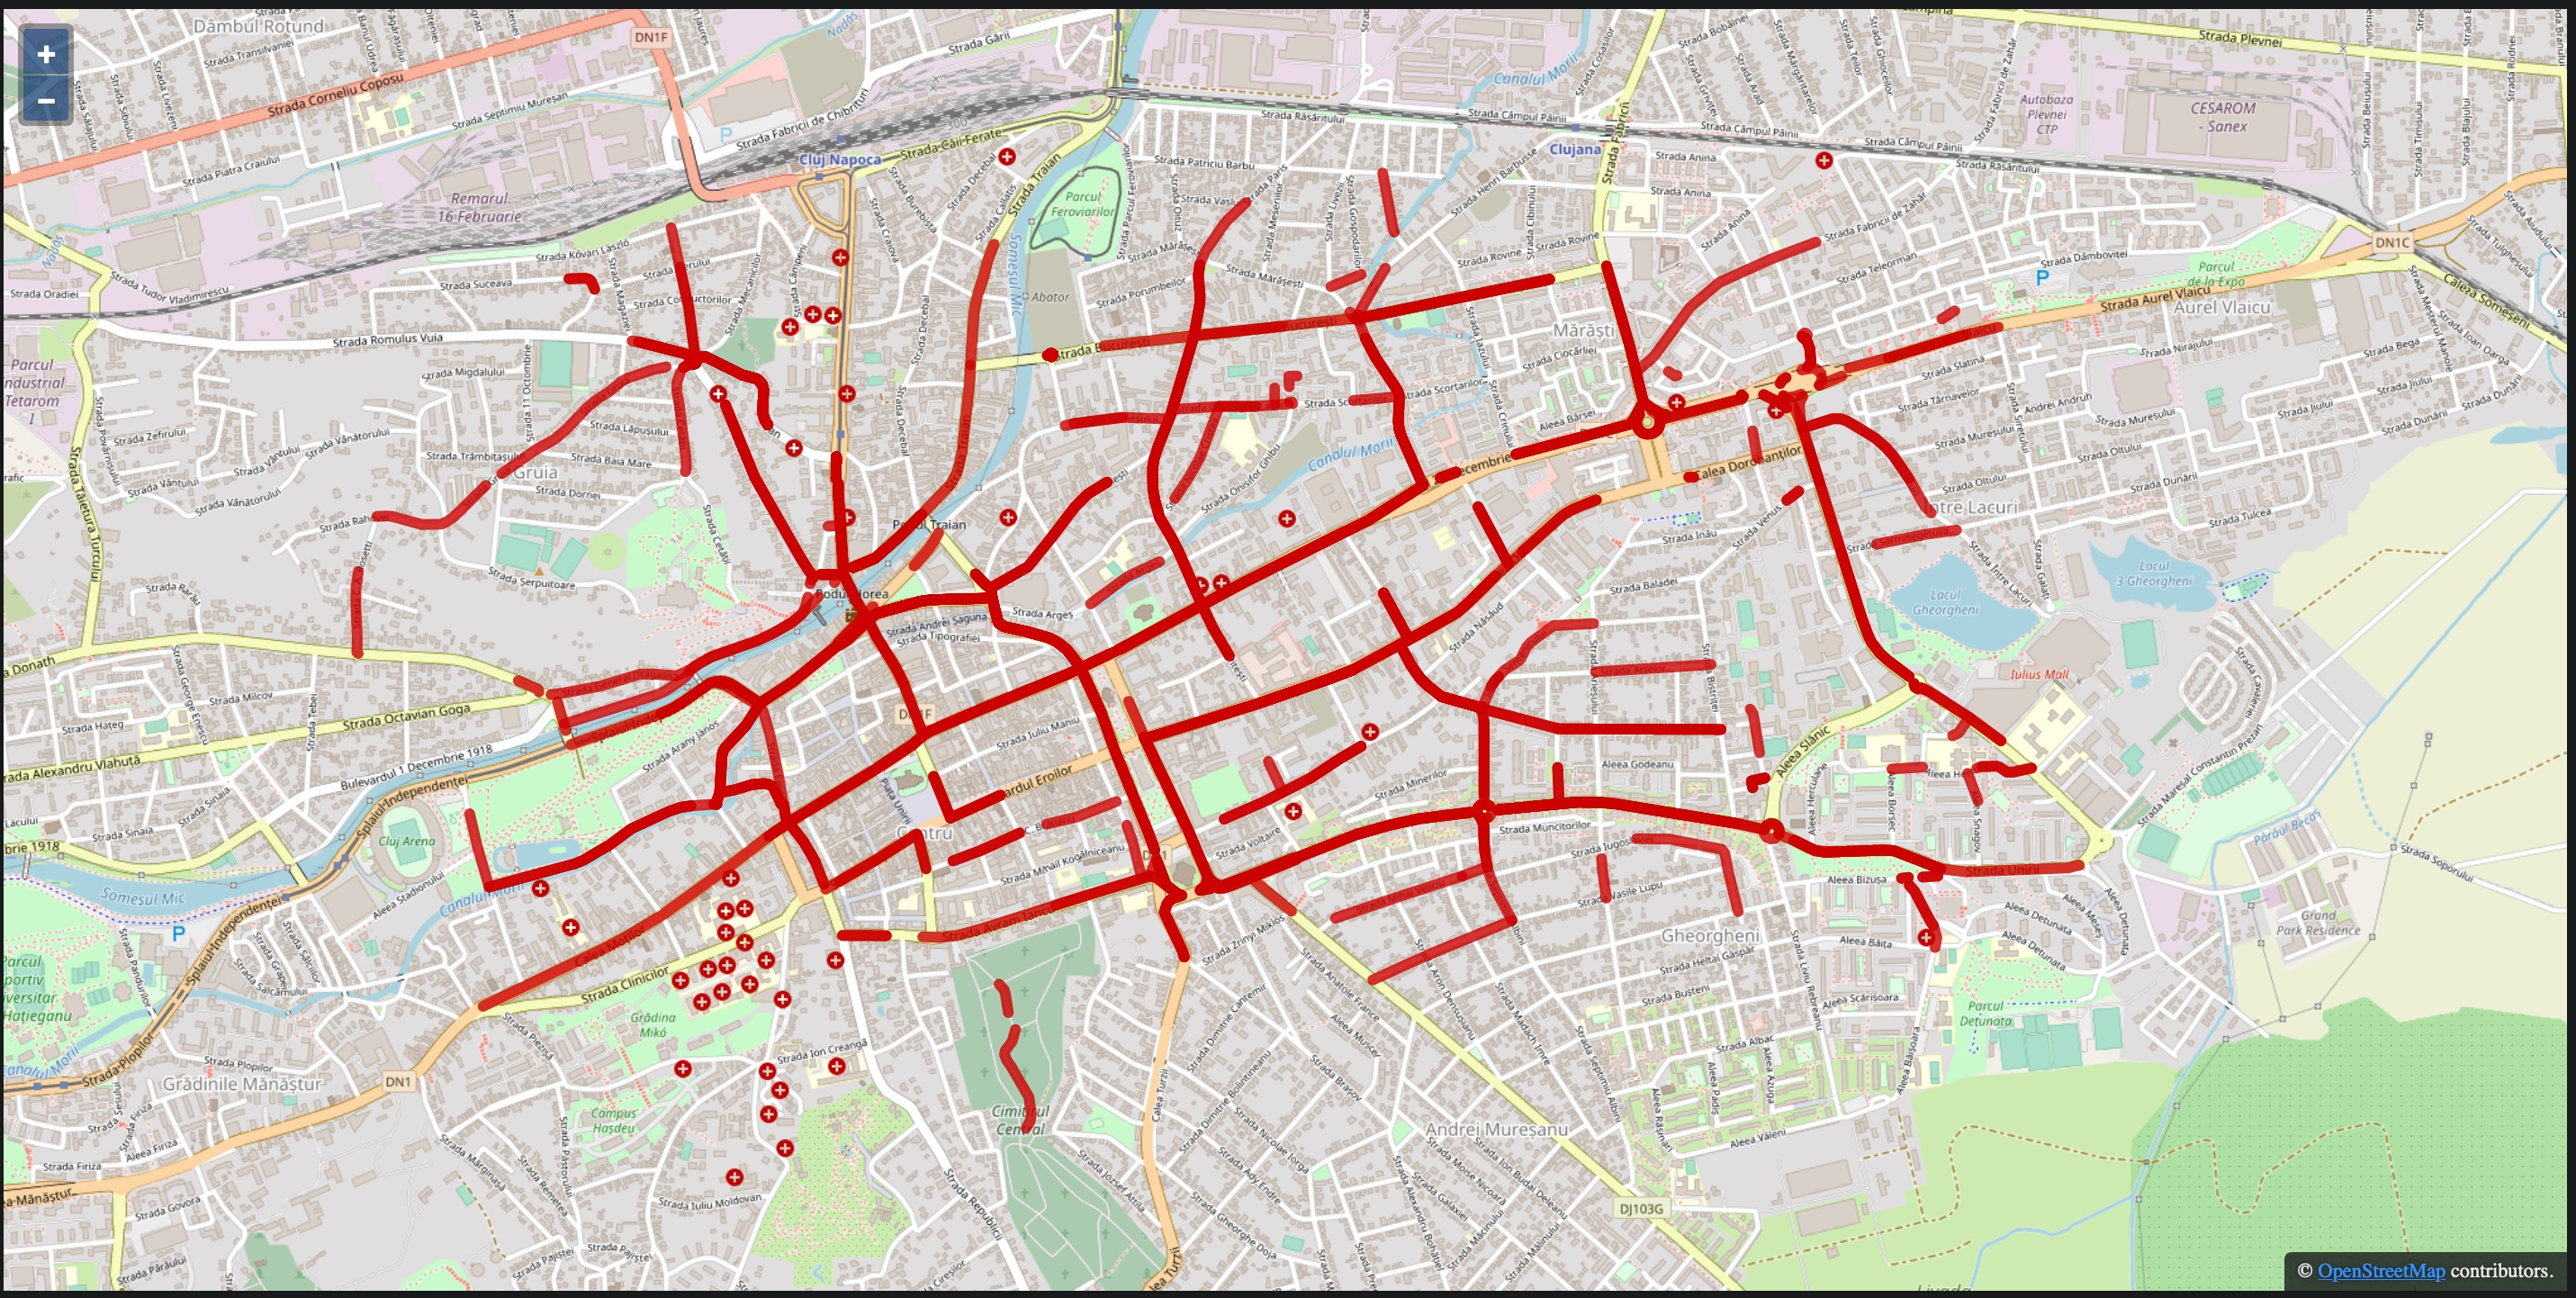
\includegraphics[width=0.9\linewidth]{ScreenshotWebInterface2.jpg}
  \centering
  \caption{Screenshot of the web interface showing the running simulation with a larger number of actors}
  \label{fig:ScreenshotWebInterface2}
\end{figure*}

\subsection{Networking design}
\label{subsec:networking}

A distributed system has to carefully design the way in which its services communicates between them. As the nature of a distributed system is to run in multiple nodes or machines, it is obvious that the communication medium between them has to be one based on TCP/IP stack. Therefore the entire modeling of networking relies on this assumption.

A simple and basic idea, noted here only to help on constructing the final proposed solution, is to have each service always located at a certain IP address and a certain port within a network. This means, for example, the city simulator will always be located at 192.168.0.101:7450. The other services which need to be accessed will listen on similar IP addresses and sockets. While this offers a convenient way to have them unified, they are not suitable to run in other environments than a development PC. In this case \textit{docker-compse} will run them such that they are accessible on local host address, i.e. 127.0.0.1:7450. As soon as there are multiple nodes involved this model is not suitable anymore.

Enter the DNS (Domain Name System), the backbone of the entire internet. In its simplest description, avoiding many inherent and nitpicking details, it is a dictionary which keeps track of every registered and easy to memorize name, e.g. \textit{en.wikipedia.com} and the IP addresses where it is located. Any client which would like to access such an name will query first the DNS resolvers and then it will proceed to send a message to the obtained IP address. The most notable interaction of a user with the DNS is the address bar of a browser where the user inserts the name of the site they want to access and while writing the address suggestions are displayed by the browser with the help of recommandation engines \cite{risley2001domain}.

When many resources are needed, to serve a great number of users or to support a great number of city actors, a certain service might be so busy with serving data that the compute and memory resources it needs are greater than the underlying hardware is able to support. Therefore it might be located at few addresses at the same time and any client which wants to access it should access the address where there are available compute and memory resources to serve its queries. Ideal would be to abstract or to decouple this information from the client and make it transparent for it. To do this the client needs to know only the service name and a certain "networking" entity should route its request to the appropiate available service. Such a entity could be a DNS authoritative server which, based on the load, availability and latency of the services will route the request to the appropiate node \cite{swildens2006scalable}.

Docker and Kubernetes are doing a similar job. They offer a DNS service and according to the load of each node where a service run, a request is rooted to a node which will be able to respond to it. This logic is completely decoupled from the clients. Listings \ref{lst:gocityclientdial} and \ref{lst:cityfrontclientdial} shows how both the city front and a city actor calls the city simulator. All what they do is to use the address, the service name, which was specified in the docker-compose file (listing \ref{lst:dockercompose}). Docker or Kubernetes will do the actual job to route the request to the appropiate node of the service. One thing to note is the difference between the two. A city client will communicate via TCP/IP using the Go default serialization package while the city front use a WebSocket communication technology (add reference to the design choices paragraph) but both of them are transparently routed by Docker.

\begin{lstlisting}[caption=City actor dialing City simulator, label=lst:gocityclientdial]
conn, err := net.Dial("tcp", "citysim:7450")
if err != nil {
    fmt.Println("Error on dialing", err)
    break
}
defer conn.Close()
\end{lstlisting}

\begin{lstlisting}[caption=City front dialing City simulator, label=lst:cityfrontclientdial]
var startWebsocket = function (callback) {

    var ws = new WebSocket("ws://citysim:9000/city")

    ws.onopen = function(evt) {
        console.log("OPEN");
        ws.send("just sent some messageeeee")
    }
    ws.onclose = function(evt) {
        console.log("CLOSE");
        ws = null;
    }
    ws.onmessage = function(evt) {
        callback(evt.data);
    }
    ws.onerror = function(evt) {
        console.log("ERROR: " + evt.data);
    }
}
\end{lstlisting}

\section{Results and evaluation}
\label{sec:results}

Fig. \ref{fig:ScreenshotWebInterface2} shows a screenshot of the web interface discussed in paragraph \ref{subsection:citysimulator}, showing a running simulation. The web interface is a simple: a html/js only web page (vanilla js) which connects to the city simulator as can be seen in listing \ref{lst:cityfrontclientdial}. The city simulator will send a notification to the web page server each time the density changes for a certain line. It can be that a new or first actor entered a certain line (a list of coordinates which represent a street) or it can be that one or the last actor left a line. The web page will draw any line with a density greater than 0 on top of the map.

The map is sourced from Open Street Map \cite{openstreetmap} and is showing the map zoomed to a specific city, same used by the city actors in their walkings. Thus, whenever a city actor reports that it is traveling across a line and this information arrives at the web interface through the city simulator, the respective line will be immediately drawn into the view.

A laptop used for simulating (MacBook Pro, 16 GB RAM, i5 3.1 GHz) is able to run easily 50 city actors. Above a certain threshold the bottleneck, surprisingly, is not the memory or the cpu but the way docker handles network interfaces. For a larger number of city actors a better tool must be used (see paragraph \ref{subsec:kubernetes}). Fig \ref{fig:ScreenshotWebInterface2} shows a simulation with 50 actors running at the same time throughout the city.

\section{Conclusions and future work}
\label{sec:enhancements}

The concept of modeling or simulating traffic using actors or agents is widespread. The advantages it offers, compared to macroscopic simulation techniques, is that more nuanced data can be obtain, usually by simulating real events and situations more easier when the agents can interact and influence each other. On top of the actor (or agent, or entity) based model, the current paper, compared with the other noted beforehand, has shown the benefits of using today's concepts of distributed systems: containers and orchestration. Those ideas (or concepts or programming frameworks), not novel in their basic traits but novel in the ease of use, enable the scaling of simulation needs across many more physical machines. In parallel with this the code being written do not suffer from leaky abstractions of the distributed nature it runs in. It is kept slim and focused, while the frameworks used are taking care of all the other networking details.

Microservices concept has been presented and together with it the city simulator and the city actor types have been introduced. Their interactions, through a specific protocol, have been presented. Moreover, various other interactions, with supporting roles (routing engine and web page) have been presented: the routing engine can be called by any actor via a REST based API and the web page keeps an open WebSocket connection towards the city simulator to be notified of any change. Design choices, lead by the programming language (Go language) and container tool (Docker) have been discussed, together with their advantages. Networking details and design have been detailed, mostly lead by how the Docker and Linux containers landscape work. Kubernetes, as the de facto solution for microservices orchestration was also presented. Finally, a brief description provided the results of a simulation run on a single machine.

\balance

As with all technical projects, there are a number of enhancements which can be further developed around the concept of simulating a city traffic through actors running in microservices, as presented in this paper. This section will briefly propose few of those details in the following paragraphs.

As the number of the actors are growing, a first bottlneck in the current architecture will be the city simulator. It is a single entity and it represents a single source of truth for the actors. To keep it as single source of truth but at the same time to scale it horizontally means that we need to introduce few additional concepts. In \cite{6847479} a first idea might be of using multiple cloud providers for taking advantage of their available compute resources and also for combining them. This would serve both to the city simulator as well to the swarm of city actors. The other part which remains is to keep the city simulator as a single source of truth by taking advantage of a distributed database. Something similar can be seen in \cite{8509417} where a NoSQL database is used for horizontally scaling. To take advantage of the Kubernetes cluster there are similar horizontally scalable databases which can be built upon. One option is the distributed key-value store used by Kubernetes itself: Etcd database \cite{etcd}.

A second idea for enhancing the simulation is to make the actors to have a more granular and diverse logic of traversing the city. The solution proposed into this paper is a basic one: an actor has a route between two random points on the map and then it goes on to travel across that route. It can also be made to look for street densities in advance and act accordingly. If a street is too crowded the actor might choose to avoid it and compute a new route around it. A set of actors can be made to always run between same points (to simulate, for example, buses).

A third idea is to add more interactions between actors. It has been discussed that a first interaction is an indirect one: the number of actors on a certain street, a number called density. But there are many more points of interactions. Let's take junctions. The city simulator can model any junction and then it can permit actors to pass or not through it, while at the same time incorporating real data as shown in \cite{urban-traffic-sim}. Then there are pedestrian crossings where different types of actors can meet each other. Or subways access, elevators for them, bus stations, etc.

A fourth idea is to have contained actors. A bus is an actor. A person is an actor. If a person is waiting on a bus station and then it takes a bus, there are two actors, but they are tied together, or contained and are not independent anymore until the actor-person choose to get out of the actor-bus. This means the densities across sidewalkings and bus stations need to be computed accordingly.

A fifth idea of enhancement is not tied to the way simulation is working but to how it is presented. The web page can display different colors based on the density of a line, offering a visual clue on it. Also it can easily show more information when the cursor is over a point of interest (a street, a junction, etc.). Or it can speed up a past simulation and it can display an animation.

\bibliographystyle{ieeetran}
\bibliography{references}

\vspace{12pt}

\end{document}
